\documentclass{article}

%%%%%%%%%%%%%%%%%%%%%%%%%%%%%%%%%%
% style template inspired from Overleaf's arXiv template:
% https://www.overleaf.com/latex/templates/style-and-template-for-preprints-arxiv-bio-arxiv/vknsbpqnxqsk
%%%%%%%%%%%%%%%%%%%%%%%%%%%%%%%%%%

\usepackage{/Users/arthur/Documents/Git/Template_Tex/arxiv_light} % see this for how to import cleanly : https://tex.stackexchange.com/questions/1137/where-do-i-place-my-own-sty-or-cls-files-to-make-them-available-to-all-my-te

\usepackage[utf8]{inputenc} % allow utf-8 input
\usepackage[T1]{fontenc}    % use 8-bit T1 fonts
\usepackage{hyperref}       % hyperlinks
\usepackage{url}            % simple URL typesetting
\usepackage{booktabs}       % professional-quality tables
\usepackage{amsfonts}       % blackboard math symbols
\usepackage{nicefrac}       % compact symbols for 1/2, etc.
\usepackage{microtype}      % microtypography
\usepackage{lipsum}

\usepackage{graphicx}

\title{Reading Notes: \cite{frankle_lottery_2018}}

\author{Arthur Roullier}

\begin{document}
\maketitle

% abstract can be removed
% \begin{abstract}
% \lipsum[1]
% \end{abstract}

% keywords can be removed
% \keywords{First keyword \and Second keyword \and More}


\section{Key Quotes}


\subsection{Abstract}
Neural network pruning techniques can reduce the parameter counts of trained net- works by over 90\%, decreasing storage requirements and improving computational performance of inference without compromising accuracy. However, contemporary experience is that the sparse architectures produced by pruning are difficult to train from the start, which would similarly improve training performance.
We find that a standard technique for pruning weights naturally uncovers subnet- works whose initializations made them capable of training effectively. Based on these results, we articulate the lottery ticket hypothesis: dense, randomly-initialized feed-forward networks contain subnetworks (winning tickets) that—when trained in isolation—arrive at comparable test accuracy in a comparable number of iterations. The winning tickets we find have won the initialization lottery: their connections have initial weights that make training particularly effective.
We present an algorithm to identify winning tickets and a series of experiments that support the lottery ticket hypothesis and the importance of these fortuitous initializations. We consistently find winning tickets that are less than 10-20\% of the size of several fully-connected and convolutional feed-forward architectures for MNIST and CIFAR10. Furthermore, the winning tickets we find above that size learn faster than the original network and exhibit higher test accuracy.


\subsection{Concepts}

\begin{itemize}
	\item 
\end{itemize}


\subsection{Results}

\begin{enumerate}
	\item \emph{The Lottery Ticket Hypothesis}. Any randomly-initialized, dense feed-forward neural network that trains to a particular test accuracy contains a subnetwork that is initialized such that—when trained in isolation—it can learn to match the accuracy of the original network after learning for at most the same number of training iterations.
	\item \emph{The Lottery Ticket Conjecture}. Returning to our motivating question, we extend our hypothesis into an untested conjecture that gradient descent seeks out and trains a subset of well-initialized weights. Randomly-initialized, unpruned networks are easier to train because they have more possible subnetworks from which training can recover a winning ticket.
	\item Contributions.
		\subitem We demonstrate that pruning uncovers sparse, trainable networks that reach test accuracy comparable to the original, feed-forward networks from which they derived.
	 	\subitem We show that winning tickets at moderate levels of pruning learn faster and reach higher test accuracy than the original network.
	 	\subitem  We propose the lottery ticket hypothesis as a new perspective on the composition of neural networks to explain these findings.
	
\end{enumerate}


\subsection{Thoughts}

\begin{itemize}
	\item  I read very quickly and it seems that the algorithm they propose to find winning tickets is not fast (see Appendix A in \cite{frankle_lottery_2018}). So it can not be used (yet?) to train a smaller network in practice. So at this point, the  Lottery Ticket Hypothesis \emph{may} be a trivial  fact, although it is interesting to state it in order to clarify the phenomenon.
	\item Another assumption, that seems true and is interesting to state that clearly, but seems of no specific interest unless we find winning tickets \emph{efficiently}:
	\begin{quote}
		We conjecture (but do not empirically show) that SGD seeks out and trains a well-initialized subnetwork. By this logic, overparameterized networks are easier to train because they have more combinations of subnetworks that are potential winning tickets.
	\end{quote}

\end{itemize}


 

\section{Diving In}

\begin{figure}[h]
	\begin{center}
		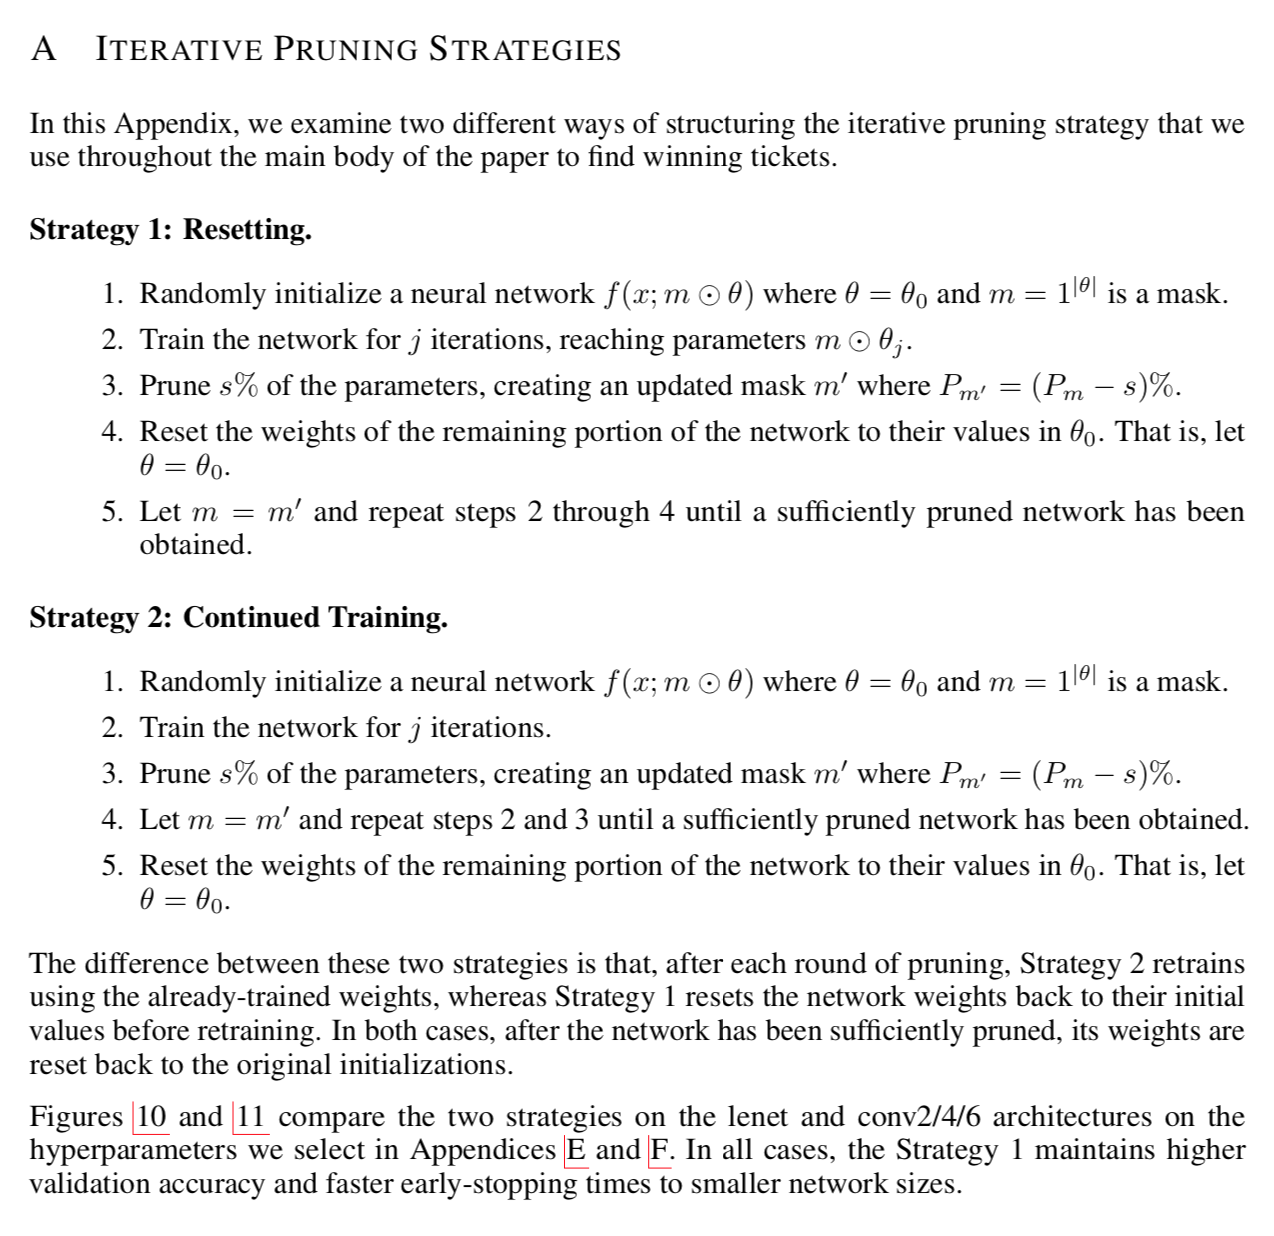
\includegraphics[width=.8\linewidth]{Figure/text_appendixA}
		%	\caption{xxx}
		\label{fig:appendixA}
	\end{center}
\end{figure}



\bibliographystyle{unsrt}
\bibliography{/Users/arthur/Documents/Git/Template_Tex/myLibrary.bib}



\end{document}
